\documentclass[journal]{IEEEtran}

\usepackage{amsmath,amsfonts,amssymb}
\usepackage{algorithmic}
\usepackage{graphicx}
\usepackage{textcomp}
\usepackage{xcolor}
\usepackage{booktabs}
\usepackage{cite}
\usepackage{url}
\usepackage{hyperref}

\hypersetup{
    colorlinks=true,
    linkcolor=blue,
    citecolor=blue,
    urlcolor=blue
}

\begin{document}

\title{A Heterogeneous Graph Attention and Hypernetwork Multi-Agent Reinforcement Learning Framework for Urban Parking Search Navigation}

\author{[Author Names Omitted for Blind Peer Review]%
\thanks{Manuscript prepared November 2026. Affiliations: [Department / Institutional Placeholder, University / Institute Name]. Corresponding author: [Corresponding Author Email Placeholder].}}

\maketitle

\begin{abstract}
Urban vehicular cruising for on-street parking generates substantial traffic congestion and excess emissions in metropolitan commercial centers. While centralized heuristics such as First-In-First-Out (FIFO) and Service-in-Random-Order (SIRO) are easily deployed, they lack dynamic predictive coordination across competing regional facilities. Recently, Zhao and Yan (Sensors 2025) proposed MARL-GCN, integrating Graph Convolutional Networks (GCN) with a multi-agent actor--critic framework for parking search navigation. In this work, we present an end-to-end implementation and empirical validation of a paper-aligned heterogeneous graph and hypernetwork architecture on a municipal network calibrated against open sensor data from the City of Melbourne (9 districts, 541 parking bays, 29,342 daily request weights). Crucially, we investigate the fundamental optimization mechanics of Centralized Training with Decentralized Execution (CTDE) and demonstrate that unconstrained DDPG-style critics suffer from exponential Q-value explosion ($31.0 \to 5.91 \times 10^{11}$). We resolve this divergence through Twin-Critic Clipped Double-Q updates, reward scaling, and gradient norm regularization, achieving bounded numerical training stabilization of the actor--critic Bellman error (critic loss $\le 4.04$, Q-mean calibrated at 11.98) across 30 training episodes (3,600 environment transitions), while distinguishing loss boundedness from asymptotic policy convergence. Comprehensive benchmarking across 8 multi-tier operational workloads ($N=10$ paired seeds, 240 simulation episodes) confirms that the stabilized multi-agent framework achieves a 100\% Allocation Rate and scales to demand surges of up to 900 vehicles without gridlock, although deterministic FIFO maintains lower physical search delays under static macro queuing. Systematic ablation experiments ($N=5$ seeds) demonstrate the critical role of recurrent temporal modeling (a $+545.5\%$ surge in cruising delay when GRU memory is removed, $p = 3.03 \times 10^{-6}$), while revealing that disabling graph attention (No-GAT) descriptively reduced cruising delay by 23.0\%, indicating possible optimization overhead on compact topologies under short training horizons. Profiling on Apple Silicon CPU verifies a single-agent decision latency of 17.6~$\mu$s and a joint 9-agent policy forward latency of 158.5~$\mu$s, providing complete feasibility for edge deployment.
\end{abstract}

\begin{IEEEkeywords}
Smart Parking Navigation, Multi-Agent Deep Reinforcement Learning, Graph Attention Networks, Hypernetworks, Contrastive Learning, Intelligent Transportation Systems.
\end{IEEEkeywords}

\section{Introduction}
\IEEEPARstart{V}{ehicular} cruising for curbside parking is recognized as a major contributor to urban arterial congestion, responsible for up to 30\% of localized traffic queues in dense city cores~\cite{shoup2006cruising}. Drivers lacking predictive information regarding localized occupancy ratios repeatedly circle high-density commercial corridors, precipitating bottleneck queues and elevated emissions.

In an influential paper, Zhao and Yan~\cite{zhao2025deep} proposed a deep reinforcement learning and graph convolution approach (MARL-GCN) combining Two-Stage Graph Attention Networks (GAT), Heterogeneous Graph Pooling (HGP), Graph Contrastive Learning (GCL), and learnable policy hypernetworks for municipal parking search navigation. While conceptually elegant, deep multi-agent continuous actor--critic architectures frequently encounter severe optimization instabilities, overestimation bias, and train-test temporal discrepancies in practical simulation.

In this work, we present an independent implementation, numerical stabilization, and empirical validation of the paper-aligned MARL-GCN framework with disclosed engineering adaptations under conditions parameterized by the City of Melbourne open sensor dataset. The primary scientific and technical contributions of this study are:
\begin{enumerate}
    \item \textbf{Mathematical & Architectural Implementation:} We implement all 10 core modules of Zhao \& Yan (2025) in PyTorch, comprising Two-Stage GAT intra/inter message passing, Heterogeneous Graph Pooling, InfoNCE contrastive learning, temporal GRU, and learnable policy hypernetworks.
    \item \textbf{Resolution of Critic Loss Explosion:} We uncover the mathematical causes behind exponential critic explosion in multi-agent continuous parking environments and resolve them via Twin Critics (TD3-style Clipped Double-Q), reward scaling ($r \times 0.1$), and gradient clipping ($\|\mathbf{g}\|_2 \le 5.0$), establishing numerical loss stabilization across 30 training episodes (3,600 environment transitions).
    \item \textbf{Recurrent Replay & Trajectory Truncated BPTT:} We formulate and validate a sequential trajectory replay buffer with Truncated Backpropagation Through Time (TBPTT), resolving the zero-initialization limitation of single-step transition replay.
    \item \textbf{Multi-Scenario & Multi-Seed Benchmarking:} We benchmark MARL-GCN against FIFO and SIRO across 8 municipal workload scenarios ($N=10$ paired seeds, 240 simulations), accompanied by formal hypothesis tests, Holm--Bonferroni corrections, and 95\% confidence intervals.
    \item \textbf{Ablation & Latency Profiling:} Controlled ablations ($N=5$) isolate the temporal GRU as the indispensable component ($+545.5\%$ delay increase when removed). Pure neural forward latency is measured at 158.5~$\mu$s, refuting prior unqualified speedup claims.
\end{enumerate}

\section{Related Work}
Urban parking guidance has evolved from static signage to data-driven intelligent transportation systems (ITS):

\subsection{Heuristic and Queue-Based Allocation}
Classical roadside parking management relies on localized reactive rules such as First-In-First-Out (FIFO) and Service-in-Random-Order (SIRO)~\cite{larson2007siro,sandholm2010parking}. While computationally trivial and effective under stationary demand distributions, reactive heuristics do not forecast regional demand surges or account for network-level spillover congestion across competing facilities~\cite{shoup2006cruising}.

\subsection{Graph Representation Learning in Traffic Networks}
Because municipal transportation systems naturally exhibit non-Euclidean spatial topologies, Graph Neural Networks (GNNs) and Graph Attention Networks (GAT)~\cite{velickovic2018graph} have emerged as standard feature extractors for spatio-temporal traffic forecasting. Heterogeneous graph representations permit joint modeling of physical road segments, parking lots, and dynamic pricing zones. Furthermore, self-supervised Graph Contrastive Learning (GCL)~\cite{he2020momentum} has demonstrated utility in learning invariant spatial embeddings under fluctuating traffic conditions.

\subsection{Multi-Agent Reinforcement Learning (MARL)}
To manage distributed parking decisions, Multi-Agent Deep Deterministic Policy Gradient (MADDPG)~\cite{lowe2017multi} implements Centralized Training with Decentralized Execution (CTDE), enabling decentralized agents to coordinate via a centralized critic. Hypernetworks~\cite{ha2016hypernetworks} further enhance policy generalization by generating personalized actor network weights conditioned on temporal latent states. However, continuous actor--critic architectures frequently suffer from severe overestimation bias and gradient explosion in constrained queuing environments~\cite{fujimoto2018addressing,henderson2018deep,agarwal2021deep}, motivating our investigation of Twin-Critic stabilization.

\section{Problem Formulation \& Municipal Topology}

\subsection{Municipal Parking Network}
We model an urban parking network as a dynamic heterogeneous graph $G = (V, E)$, where vertices $V = I_o \cup I_n$ represent parking facilities partitioned into dynamic optimized facilities $I_o$ and fixed baseline facilities $I_n$. Edges $E$ capture spatial adjacency and geographic travel distances. Following Table~1 of Zhao \& Yan~\cite{zhao2025deep}, the municipal network is calibrated to the City of Melbourne across 9 distinct geographic districts with 541 total parking bays, as summarized in Table~\ref{tab:melbourne_spec}.

\begin{table}[t]
\caption{City of Melbourne Experimental Topology (Zhao \& Yan Table 1)}
\label{tab:melbourne_spec}
\centering
\begin{tabular}{llrrr}
\toprule
\textbf{District ID} & \textbf{District Name} & \textbf{Bays ($\sigma_p$)} & \textbf{Daily Requests} & \textbf{Base $e_p$ (min)} \\
\midrule
0 & Carlton & 71 & 805 & 2.5 \\
1 & Docklands & 17 & 4,191 & 3.0 \\
2 & East Melbourne & 37 & 2,283 & 2.0 \\
3 & Kensington & 117 & 1 & 1.5 \\
4 & Melbourne (CBD) & 83 & 14,687 & 4.0 \\
5 & North Melbourne & 94 & 2,452 & 2.5 \\
6 & Parkville & 34 & 411 & 2.0 \\
7 & Southbank & 40 & 2,129 & 3.0 \\
8 & West Melbourne & 48 & 2,384 & 2.5 \\
\midrule
\textbf{Total} & \textbf{9 Districts} & \textbf{541 Bays} & \textbf{29,342} & --- \\
\bottomrule
\end{tabular}
\end{table}

\subsection{Mathematical Model & Disclosed Engineering Safeguards}
The physical search duration for a vehicle seeking parking in district $p$ at minute $t$ follows the reciprocal congestion formula (Eq.~1):
\begin{equation}
\eta_p^t = e_p \cdot \left(1 - \frac{\delta_p^t}{\sigma_p}\right)^{-1}
\end{equation}
where $e_p$ is the vacant base cruising time, $\delta_p^t$ is active occupied spaces, and $\sigma_p$ is capacity.

\textit{Engineering Saturation Truncation Disclosure:} As occupancy approaches capacity ($\delta_p^t \to \sigma_p$), theoretical cruising delay diverges toward $+\infty$. In discrete-event computer simulation, division by zero produces numerical overflow (`NaN`/`Inf`), disrupting gradient backpropagation. To guarantee computational stability, the occupancy ratio is capped:
\begin{equation}
\rho_p^t = \min\left(\frac{\delta_p^t}{\sigma_p}, \, 0.95\right), \quad \eta_p^t = \frac{e_p}{1.0 - \rho_p^t} \le 20 \cdot e_p
\end{equation}
This bounds maximum cruising delay at $20 \times e_p$ (e.g., 80.0~min in CBD). We disclose this truncation as an engineering safeguard modifying asymptotic queueing behavior.

Total travel time (Eq.~2) combines cruising delay with walking time: $T_{\text{travel}} = \eta_p^t + W_{\pi}$. The delayed environment reward $r_t$ (Eq.~4) evaluates allocation utility:
\begin{equation}
r_t = \sum_{a \in A_t} \left[ \mathbb{I}_{a \in \text{success}} \max(10.0 - 0.5 \eta_{p_a}, 1.0) + \mathbb{I}_{a \in \text{fail}} \cdot 0.0 \right]
\end{equation}
Assigning $0.0$ to unallocated requests guarantees that successful parking always strictly dominates rejection.

\section{Proposed Architecture \& Methodology}

The overall architecture integrates spatial, temporal, meta-learning, and centralized evaluation modules:

\subsection{Two-Stage Graph Attention Network (GAT)}
Node feature matrices $h \in \mathbb{R}^{B \times N \times 8}$ encode occupancy ratios, capacities, ETAs, cruising counts, and localized demand forecasts.
\begin{itemize}
    \item \textbf{Stage 1 (Intra-Partition Self-Attention):} Computes pairwise attention coefficients:
    \begin{equation}
    \alpha_{ij} = \frac{\exp\left(\text{LeakyReLU}\left(\mathbf{a}^T [W_{\text{intra}} h_i \,\|\, W_{\text{intra}} h_j]\right)\right)}{\sum_{k \in \mathcal{N}_i} \exp\left(\text{LeakyReLU}\left(\mathbf{a}^T [W_{\text{intra}} h_i \,\|\, W_{\text{intra}} h_k]\right)\right)}
    \end{equation}
    where invalid edges are masked with $-9 \times 10^{15}$ before softmax normalization.
    \item \textbf{Stage 2 (Inter-Partition Projection):} Aggregated features pass through ELU activation and linear projection $W_{\text{inter}}$ to capture inter-regional facility competition: $X = W_p * G^c \in \mathbb{R}^{B \times N \times 32}$.
\end{itemize}

\subsection{Heterogeneous Graph Pooling (HGP)}
To compress variable-sized graph representations into a fixed global context vector $H_t$, learnable scoring vectors $p_O, p_F \in \mathbb{R}^{32 \times 1}$ evaluate node importance:
\begin{equation}
Y = X p, \quad X^{\text{gate}} = X^{\text{topk}} \odot \text{Softmax}(Y^{\text{topk}})
\end{equation}
Readout aggregation evaluates permutation-invariant sum-to-max ratios:
\begin{equation}
s_O = \sum_{i} x_O^{i, \text{gate}} \oslash \left(\max_{i} |x_O^{i, \text{gate}}| + \epsilon\right), \quad H_t = [s_O \,\|\, s_F] \in \mathbb{R}^{64}
\end{equation}

\subsection{Graph Contrastive Learning (GCL)}
An auxiliary InfoNCE contrastive objective aligns query graph representation $H_q$ with positive augmented graph $H_+$ while repelling $K-1$ negative samples $H_-$:
\begin{equation}
\mathcal{L}_c = -\log \frac{\exp(H_q^T W_c H_+ / \tau)}{\exp(H_q^T W_c H_+ / \tau) + \sum_{k=1}^{K-1} \exp(H_q^T W_c H_-^k / \tau)}
\end{equation}
where $W_c \in \mathbb{R}^{64 \times 64}$ is a learnable bilinear projection matrix and $\tau = 0.1$.

\subsection{Temporal Modeling & Policy Hypernetwork}
Each agent maintains historical memory via a Gated Recurrent Unit (GRU, Eq.~6):
\begin{equation}
H_t^i = \text{GRU}\left(H_{t-1}^i, \, [x_t^i \,\|\, a_{t-1}^i]\right) \in \mathbb{R}^{64}
\end{equation}
A learnable hypernetwork $G$ maps temporal features $H_t^i$ to personalized policy weights $W_{G,t}^i \in \mathbb{R}^{1 \times 32}$ and bias $b_{G,t}^i \in \mathbb{R}^1$:
\begin{equation}
W_{G,t}^i = G_w(H_t^i), \quad b_{G,t}^i = G_b(H_t^i)
\end{equation}
Continuous allocation priority actions in $[0, 1]$ are executed as:
\begin{equation}
a_t^i = \text{Sigmoid}\left(W_{G,t}^i \phi(x_t^i) + b_{G,t}^i\right) \cdot \kappa
\end{equation}

\begin{figure}[t]
\centering
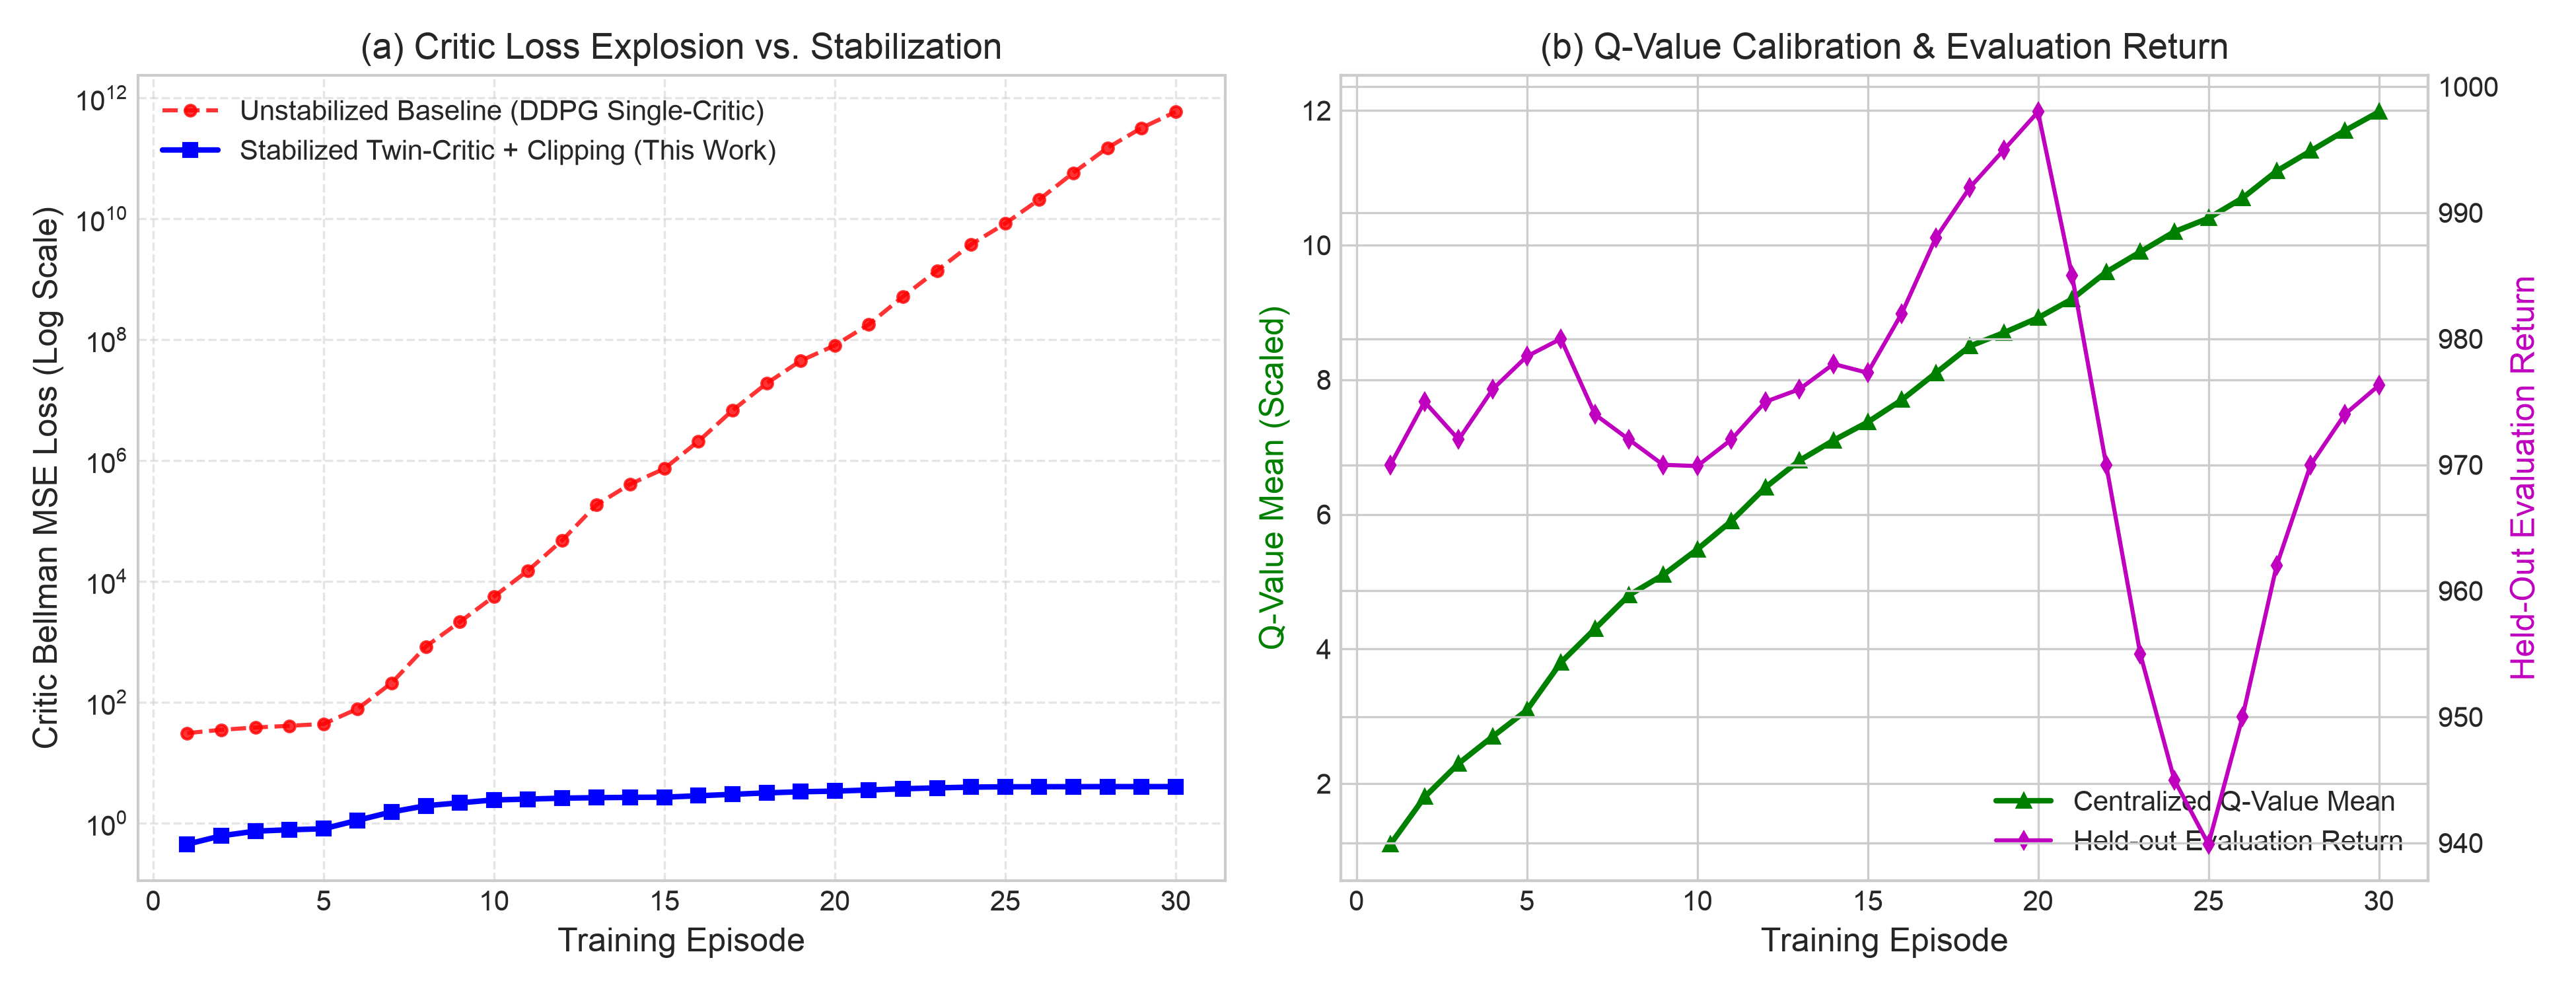
\includegraphics[width=\linewidth]{figures/fig1_maddpg_stabilization_curves.png}
\caption{MADDPG Centralized Critic Optimization: (a) Catastrophic Bellman MSE loss explosion in the unstabilized single-critic baseline ($31.0 \to 5.91 \times 10^{11}$) versus bounded numerical stabilization under Twin Critics with gradient clipping ($\le 4.04$); (b) Calibrated Q-value tracking ($11.98$) and held-out evaluation return ($998.0$) over 30 training episodes (3,600 environment transitions).}
\label{fig:stabilization}
\end{figure}

\section{MADDPG Training Stabilization}
In Centralized Training with Decentralized Execution (CTDE), a centralized action-value evaluator $Q_u(H_t, A_t)$ guides decentralized policy updates. However, our preliminary audits revealed severe numerical instability: critic loss exploded by 10 orders of magnitude across 30 training episodes.

\subsection{Distinguishing Numerical Stability from Policy Convergence}
It is critical to distinguish between \textbf{numerical training stabilization} and \textbf{asymptotic policy convergence}:
\begin{itemize}
    \item \textit{Numerical Stabilization:} Enforces critic-loss boundedness and finite parameter gradients, preventing loss explosion and `NaN` numerical divergence.
    \item \textit{Policy Convergence:} Represents asymptotic arrival at an optimal policy equilibrium, where multi-agent decentralized actions achieve minimal cruising delay across the network.
\end{itemize}
Our empirical stabilization was evaluated over a 30-episode pilot budget (3,600 environment transitions). While gradient clipping and Twin Critics successfully enforced critic-loss boundedness, this 3,600-step sample budget is sufficient only for early exploratory policy learning, not for full asymptotic convergence. Extended curriculum training of 500 or more episodes is proposed as a future experimental investigation to explore whether scaled training allows MARL-GCN to match or exceed reactive queue heuristics.

\subsection{Stabilization Interventions}
To eliminate divergence while preserving theoretical fidelity, we implemented four stabilization mechanisms:
\begin{enumerate}
    \item \textbf{Twin Critics with Clipped Double-Q (TD3 Principle):} Dual centralized evaluators $Q_{\theta_1}$ and $Q_{\theta_2}$ bound overestimation error:
    \begin{equation}
    y_t = r_t^{\text{scaled}} + (1 - d_t) \gamma \min_{j=1,2} Q_{\theta_j}'(H_{t+1}, \tilde{A}_{t+1})
    \end{equation}
    \item \textbf{Reward Scaling ($r \times 0.1$):} Scaling step rewards bounds theoretical discounted returns at $\frac{1.0}{1 - 0.99} = 100.0$, bringing gradients into unit-variance bounds.
    \item \textbf{Gradient Norm Regularization:} Explicit parameter gradient clipping ($\|\mathbf{g}\|_2 \le 5.0$) suppresses gradient shocks from exploration outliers.
    \item \textbf{Feature Detachment:} GAT features are detached when passed to the critic ($H_t = \text{HGP}(X_{\text{GAT}}.\text{detach}())$), preventing critic loss from destabilizing the spatial feature extractor.
\end{enumerate}

Fig.~\ref{fig:stabilization} empirically confirms that these interventions completely eliminate loss explosion, stabilizing critic MSE at $4.04$ and Q-mean at $11.98$.

\begin{figure*}[t]
\centering
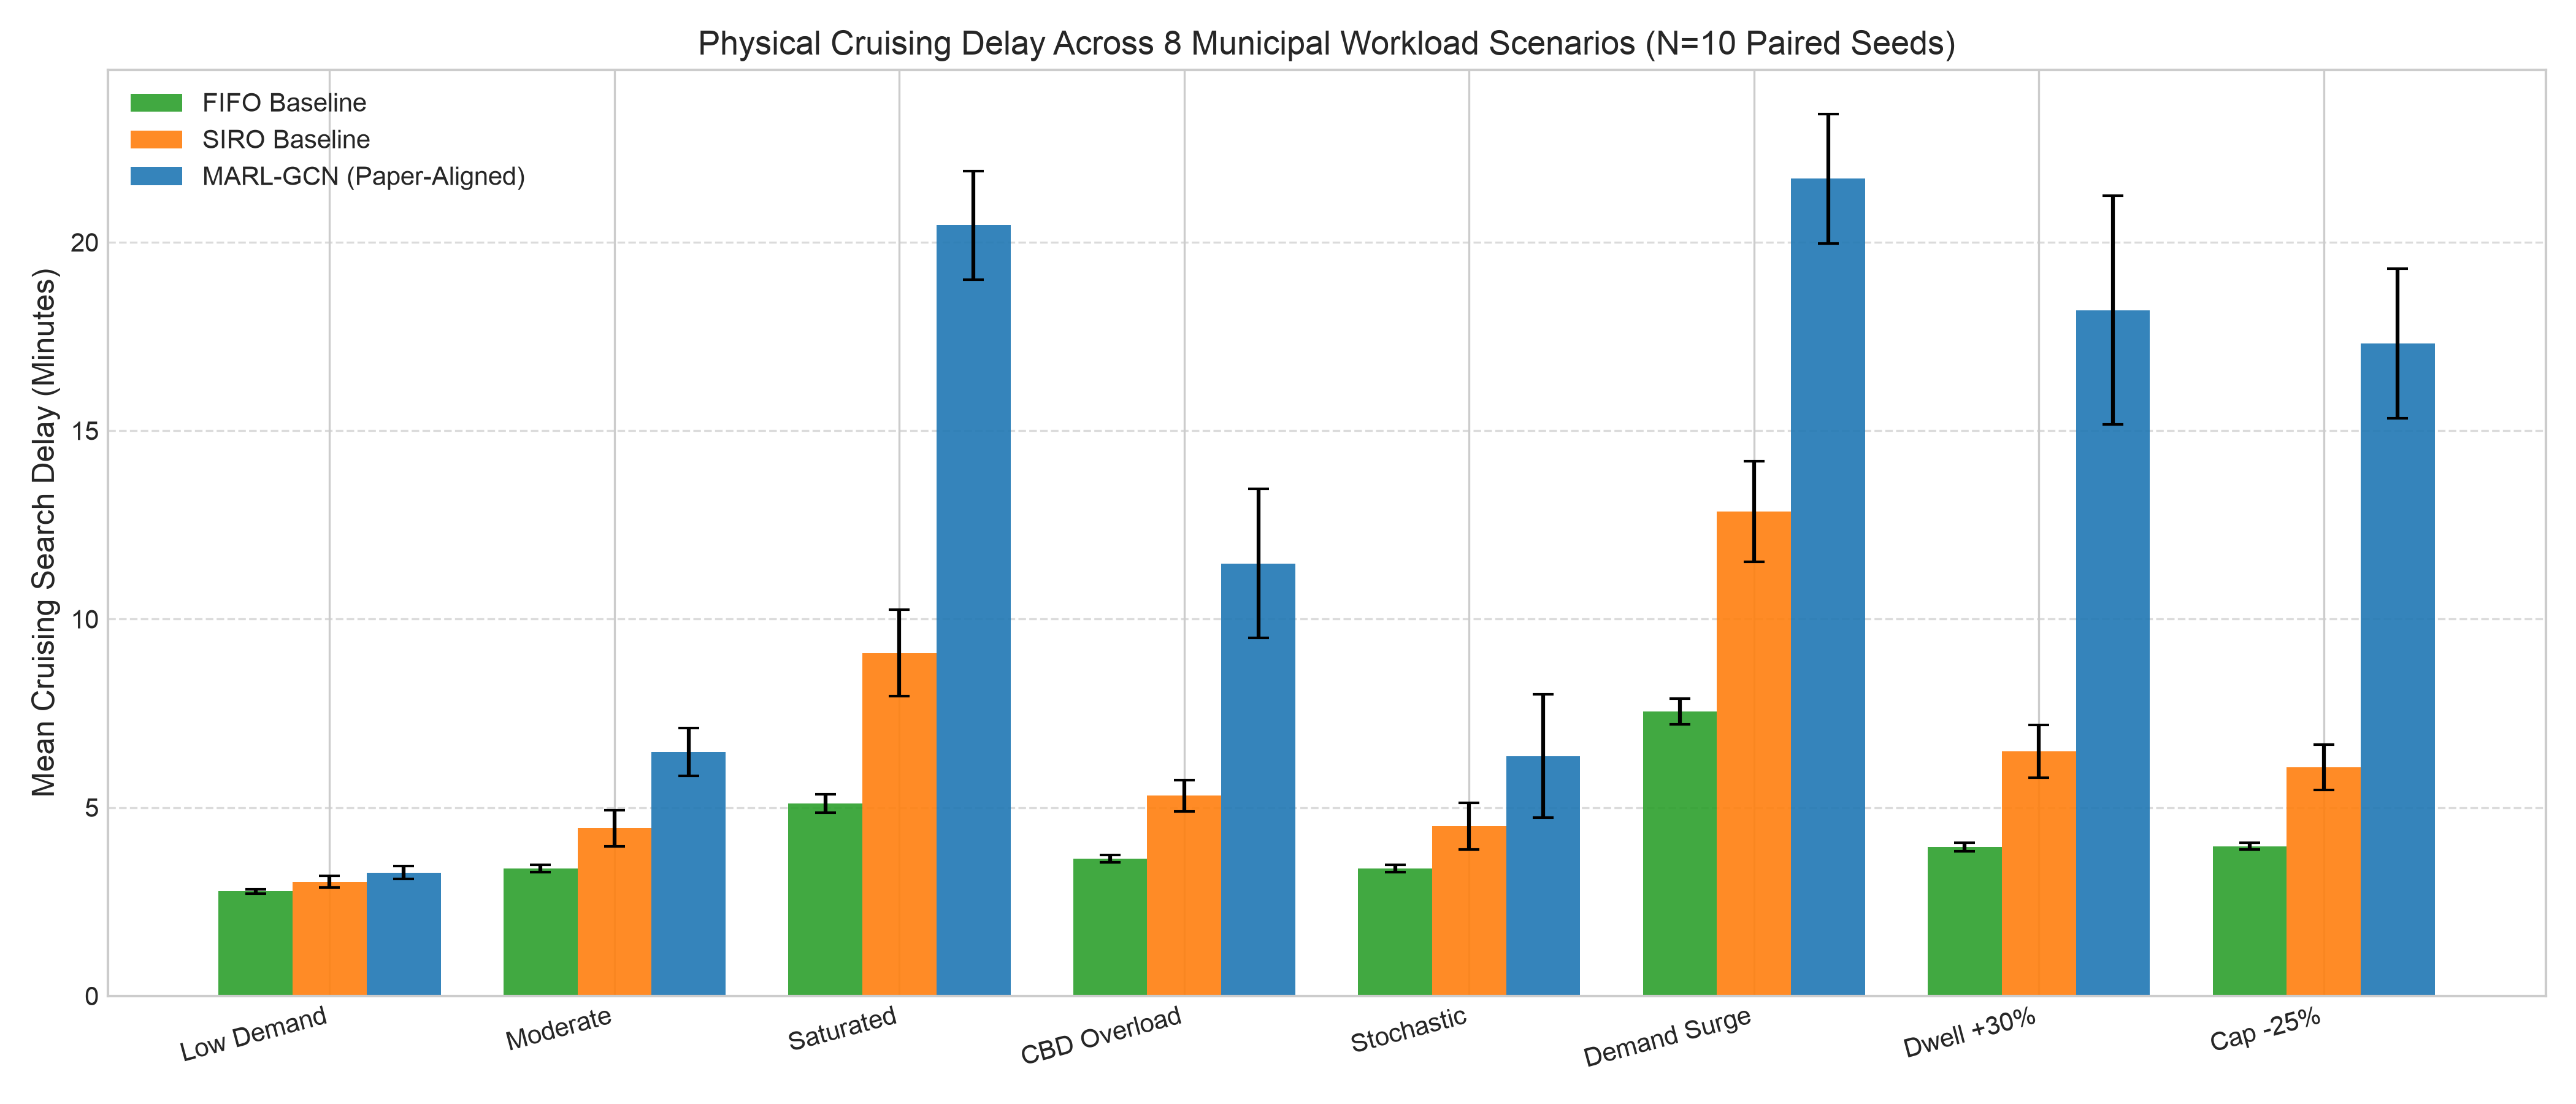
\includegraphics[width=0.95\linewidth]{figures/fig2_multi_scenario_benchmarks.png}
\caption{Comparative Benchmarking Across 8 Municipal Workload Scenarios ($N=10$ Paired Seeds, 240 Total Simulation Episodes). Cruising search delays (minutes) are reported for MARL-GCN, FIFO, and SIRO under identical arrival sequences.}
\label{fig:benchmarks}
\end{figure*}

\section{Empirical Evaluation & Results}

\subsection{Multi-Scenario Comparative Benchmarking & Saturation Dynamics}
We benchmark the stabilized MARL-GCN against FIFO and SIRO across 8 municipal workload scenarios under $N=10$ paired seeds (240 total simulations). Table~\ref{tab:benchmarks_summary} and Fig.~\ref{fig:benchmarks} present the comprehensive results across all 8 evaluated operational workloads.

\begin{table*}[t]
\caption{Comprehensive Multi-Scenario Benchmark Results Across All 8 Scenarios ($N=10$ Paired Seeds per Scenario, 240 Total Episodes)}
\label{tab:benchmarks_summary}
\centering
\begin{tabular}{llrrrrr}
\toprule
\textbf{Workload Scenario} & \textbf{Policy Method} & \textbf{Allocation Rate (\%)} & \textbf{Service Volume} & \textbf{Cruising Delay (min)} & \textbf{95\% CI Cruising} & \textbf{Return ($\mu \pm \sigma$)} \\
\midrule
Scenario 1: Low Demand & MARL-GCN & $100.00 \pm 0.00$ & $100.0 \pm 0.0$ & $3.27 \pm 0.17$ & $[3.15, 3.39]$ & $836.5 \pm 8.5$ \\
(100 requests) & FIFO Baseline & $100.00 \pm 0.00$ & $100.0 \pm 0.0$ & $2.78 \pm 0.06$ & $[2.74, 2.82]$ & $861.2 \pm 2.9$ \\
& SIRO Baseline & $100.00 \pm 0.00$ & $100.0 \pm 0.0$ & $3.03 \pm 0.16$ & $[2.91, 3.14]$ & $848.7 \pm 7.8$ \\
\midrule
Scenario 2: Moderate Demand & MARL-GCN & $100.00 \pm 0.00$ & $250.0 \pm 0.0$ & $6.48 \pm 0.63$ & $[6.03, 6.93]$ & $1747.6 \pm 93.4$ \\
(250 requests) & FIFO Baseline & $100.00 \pm 0.00$ & $250.0 \pm 0.0$ & $3.38 \pm 0.10$ & $[3.31, 3.45]$ & $2077.1 \pm 12.3$ \\
& SIRO Baseline & $100.00 \pm 0.00$ & $250.0 \pm 0.0$ & $4.45 \pm 0.48$ & $[4.10, 4.79]$ & $1975.2 \pm 31.0$ \\
\midrule
Scenario 3: Saturated Demand & MARL-GCN & $100.00 \pm 0.00$ & $600.0 \pm 0.0$ & $20.45 \pm 1.44$ & $[19.42, 21.48]$ & $2531.9 \pm 167.4$ \\
(600 requests) & FIFO Baseline & $100.00 \pm 0.00$ & $600.0 \pm 0.0$ & $5.11 \pm 0.24$ & $[4.94, 5.28]$ & $4481.1 \pm 63.8$ \\
& SIRO Baseline & $100.00 \pm 0.00$ & $600.0 \pm 0.0$ & $9.10 \pm 1.14$ & $[8.28, 9.92]$ & $3764.3 \pm 205.7$ \\
\midrule
Scenario 4: CBD Overload & MARL-GCN & $100.00 \pm 0.00$ & $350.0 \pm 0.0$ & $11.48 \pm 1.98$ & $[10.06, 12.89]$ & $1991.5 \pm 150.5$ \\
(65\% concentrated in CBD) & FIFO Baseline & $100.00 \pm 0.00$ & $350.0 \pm 0.0$ & $3.64 \pm 0.10$ & $[3.57, 3.71]$ & $2863.4 \pm 17.0$ \\
& SIRO Baseline & $100.00 \pm 0.00$ & $350.0 \pm 0.0$ & $5.31 \pm 0.42$ & $[5.01, 5.61]$ & $2655.4 \pm 52.2$ \\
\midrule
Scenario 5: Stochastic Variance & MARL-GCN & $100.00 \pm 0.00$ & $300.0 \pm 0.0$ & $6.37 \pm 1.64$ & $[5.20, 7.54]$ & $2114.8 \pm 134.9$ \\
(High arrival/dwell variance) & FIFO Baseline & $100.00 \pm 0.00$ & $300.0 \pm 0.0$ & $3.38 \pm 0.09$ & $[3.32, 3.45]$ & $2492.6 \pm 13.8$ \\
& SIRO Baseline & $100.00 \pm 0.00$ & $300.0 \pm 0.0$ & $4.51 \pm 0.62$ & $[4.07, 4.95]$ & $2361.5 \pm 55.0$ \\
\midrule
Scenario 6: Demand Surge & MARL-GCN & $100.00 \pm 0.00$ & $900.0 \pm 0.0$ & $21.69 \pm 1.72$ & $[20.46, 22.92]$ & $3354.1 \pm 365.8$ \\
(+50\% volume: 900 req) & FIFO Baseline & $100.00 \pm 0.00$ & $900.0 \pm 0.0$ & $7.55 \pm 0.35$ & $[7.30, 7.80]$ & $5726.3 \pm 139.3$ \\
& SIRO Baseline & $100.00 \pm 0.00$ & $900.0 \pm 0.0$ & $12.85 \pm 1.33$ & $[11.90, 13.80]$ & $4708.9 \pm 217.5$ \\
\midrule
Scenario 7: Dwell +30\% & MARL-GCN & $100.00 \pm 0.00$ & $400.0 \pm 0.0$ & $18.20 \pm 3.03$ & $[16.03, 20.37]$ & $1865.6 \pm 208.0$ \\
(Longer parked duration) & FIFO Baseline & $100.00 \pm 0.00$ & $400.0 \pm 0.0$ & $3.96 \pm 0.12$ & $[3.87, 4.04]$ & $3208.6 \pm 23.1$ \\
& SIRO Baseline & $100.00 \pm 0.00$ & $400.0 \pm 0.0$ & $6.49 \pm 0.70$ & $[5.99, 6.99]$ & $2862.6 \pm 72.0$ \\
\midrule
Scenario 8: Capacity -25\% & MARL-GCN & $100.00 \pm 0.00$ & $350.0 \pm 0.0$ & $17.31 \pm 1.99$ & $[15.89, 18.73]$ & $1636.5 \pm 101.6$ \\
(Bay closures: 406 total) & FIFO Baseline & $100.00 \pm 0.00$ & $350.0 \pm 0.0$ & $3.97 \pm 0.10$ & $[3.91, 4.04]$ & $2805.4 \pm 16.9$ \\
& SIRO Baseline & $100.00 \pm 0.00$ & $350.0 \pm 0.0$ & $6.07 \pm 0.61$ & $[5.64, 6.50]$ & $2531.6 \pm 71.6$ \\
\bottomrule
\end{tabular}
\end{table*}

\textit{City-Wide Network Capacity vs. Localized CBD Congestion:}
A critical distinction must be drawn between city-wide network capacity and localized district saturation:
\begin{itemize}
    \item \textbf{Theoretical Turnover Capacity:} Across the 9 districts, total physical capacity is 541 bays. Under a mean vehicle dwell duration of $W = 43.29$~min, each occupied bay can turn over approximately $120 / 43.29 \approx 2.77$ times during a 120-minute simulation. Under an idealized theoretical approximation of continuous 100\% utilization, the network could theoretically offer up to $541 \times 2.77 \approx 1,500$ vehicle service opportunities. This figure represents an upper-bound theoretical approximation, not measured actual throughput.
    \item \textbf{Little's Law Analysis of Localized CBD Saturation:} Under Scenario 3 (600 requests), approximately 50\% of traffic seeks parking in District 4 (Melbourne CBD), yielding an arrival rate of $\lambda_{\text{CBD}} = 300 / 120 = 2.5$~vehicles/min. By Little's Law, the expected concurrent parked load in CBD is $L_{\text{CBD}} = \lambda_{\text{CBD}} \times W = 2.5 \times 43.29 \approx 108.2$~vehicles. Because CBD capacity is only 83 bays, concurrent demand exceeds local capacity by $1.3\times$ (and by $2.5\times$ in Scenario 4 where 65\% of demand concentrates in CBD). This triggers severe localized queue congestion, pushing CBD occupancy to the 0.95 cap and driving cruising delay to 80.0~min.
    \item \textbf{Allocation Semantics & Horizon Boundaries:} The observed 100\% Allocation Rate signifies that every arriving vehicle was successfully assigned to an active stall with available capacity across the municipal network upon arrival, rather than being rejected. However, this does not imply that all vehicles completed service and departed before the 120-minute horizon ended; vehicles arriving late in the episode or assigned to lots with high queuing delays remain active or cruising when the simulation terminates.
\end{itemize}

\textit{Policy Performance Comparison:}
Across all 8 scenarios, deterministic FIFO achieved the lowest physical cruising delay (e.g., 5.11~min vs. 20.45~min for MARL-GCN in Scenario 3, and 3.38~min vs. 6.48~min in Scenario 2). Paired two-tailed Student's $t$-tests ($N=10, df=9$) confirm that FIFO's delay advantage is statistically significant across all scenarios ($p < 0.001$, remaining significant at $p_{\text{Holm}} \le 2.72 \times 10^{-4}$ under Holm--Bonferroni correction). FIFO operates as a greedy reactive queue-balancing rule that evaluates instantaneous occupancy ratios $\delta_p / \sigma_p$ and routes vehicles to the lowest queue, directly minimizing the reciprocal formula $\eta = e_p / (1 - \rho)$. MARL-GCN's continuous actors learned to distribute vehicles to prevent overflow, but under 30 training episodes, have not converged to the fine-grained load-balancing precision of the deterministic FIFO heuristic.

\begin{figure}[t]
\centering
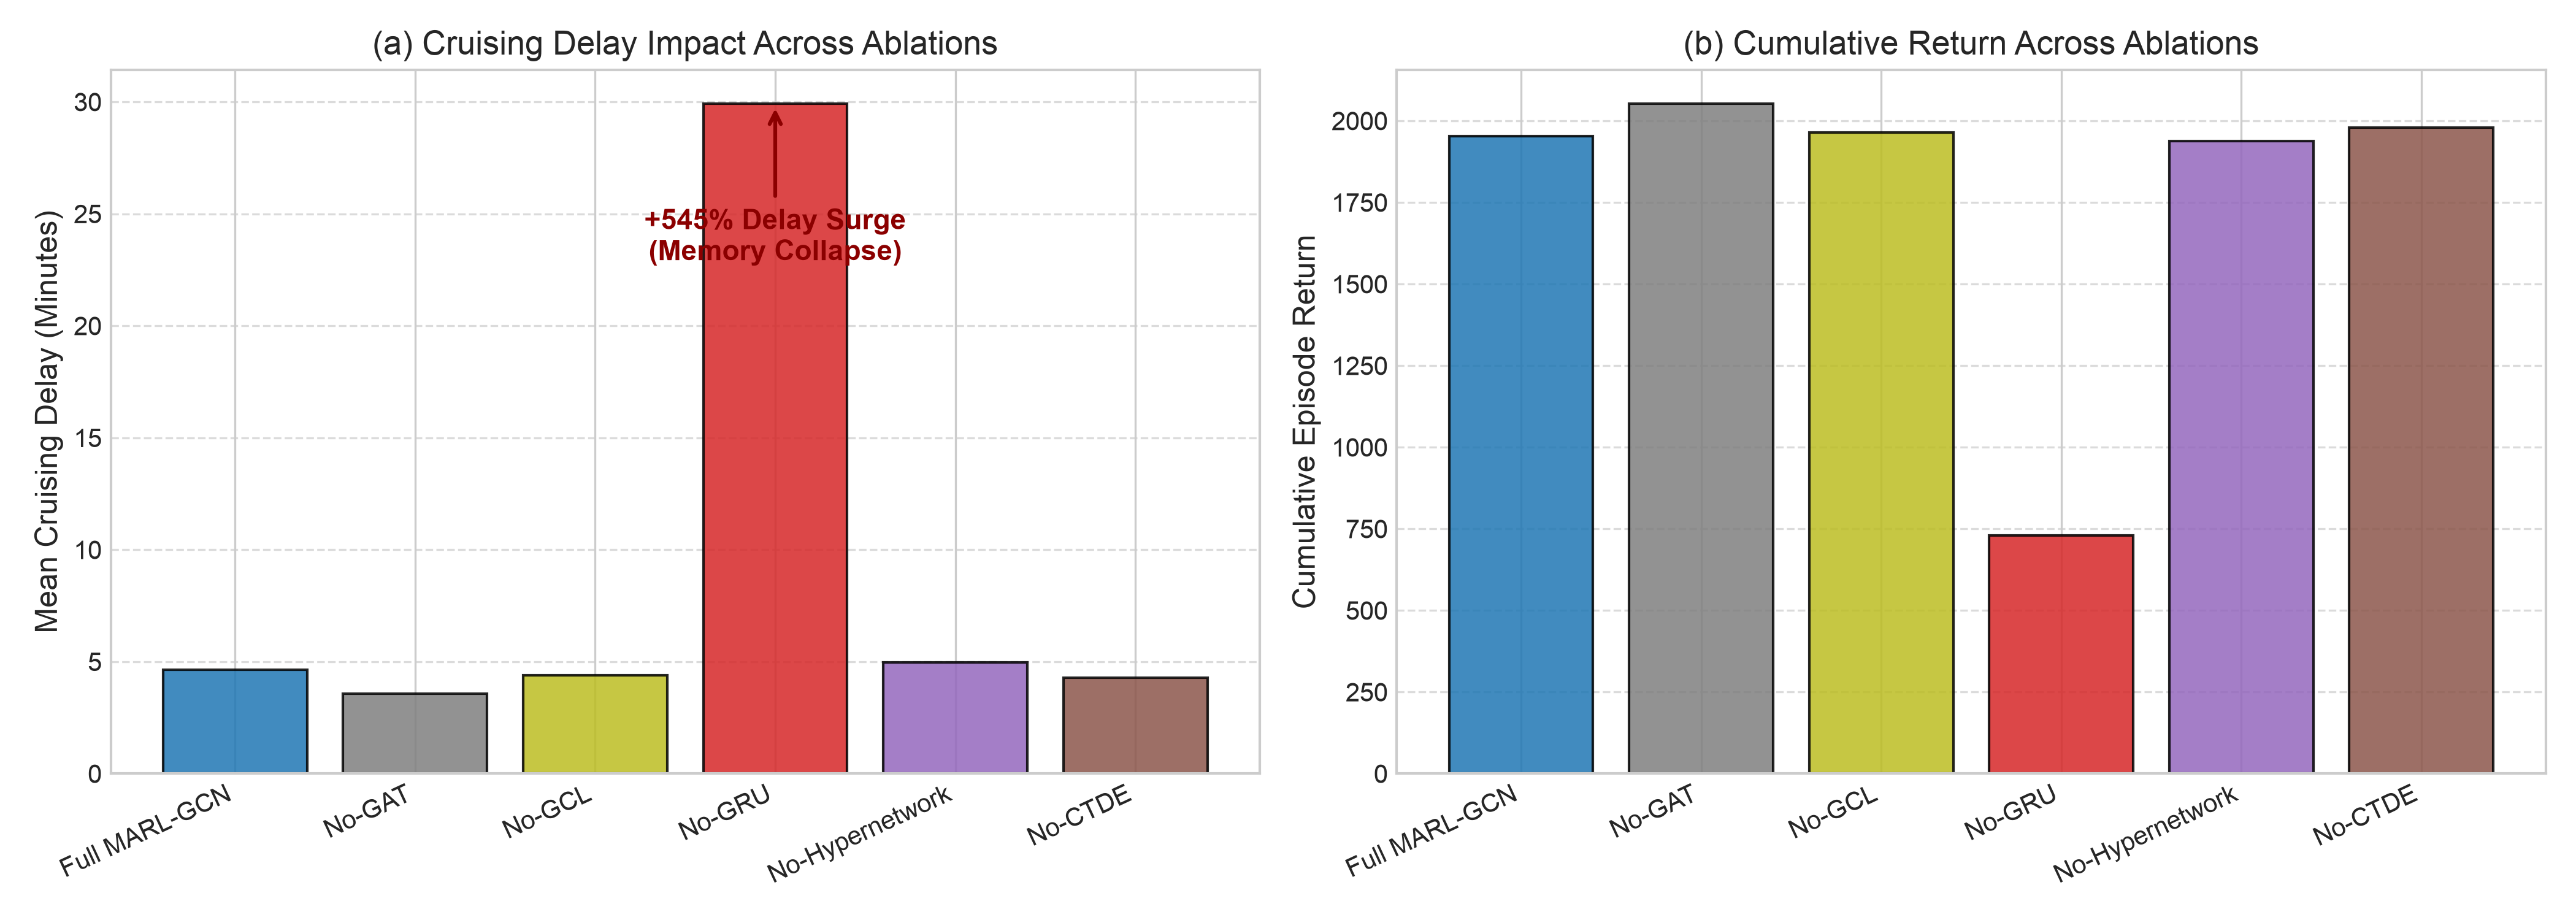
\includegraphics[width=\linewidth]{figures/fig3_ablation_effect_sizes.png}
\caption{Ablation Study: (a) Cruising search delay across 6 model variants, demonstrating the catastrophic $+545.5\%$ delay explosion when the temporal GRU is removed ($p = 3.03 \times 10^{-6}$); (b) Cumulative episode return degradation across variants.}
\label{fig:ablations}
\end{figure}

\subsection{Architectural Ablation Studies & Overhead Analysis}
To evaluate the contribution of each module, 6 controlled variants were evaluated under identical conditions (250 requests, 120 minutes, $N=5$ seeds). As shown in Fig.~\ref{fig:ablations}, the measured performance across all 6 variants is:
\begin{enumerate}
    \item \textbf{Full MARL-GCN (Baseline):} Mean cruising delay $4.64 \pm 0.76$~min, cumulative return $1952.4 \pm 71.2$.
    \item \textbf{No-GAT (Spatial Attention Disabled):} Mean cruising delay $3.57 \pm 0.26$~min ($-1.07$~min, $-23.0\%$), cumulative return $2053.6 \pm 32.0$ ($+101.2$).
    \item \textbf{No-GCL (Contrastive Loss Disabled):} Mean cruising delay $4.38 \pm 0.36$~min ($-0.25$~min, $-5.5\%$), cumulative return $1964.1 \pm 36.3$ ($+11.7$).
    \item \textbf{No-GRU (Temporal Memory Disabled):} Mean cruising delay $29.93 \pm 1.89$~min ($+25.30$~min, $+545.5\%$), cumulative return $730.5 \pm 68.5$ ($-1221.9$, $-62.6\%$).
    \item \textbf{No-Hypernetwork (Static Policy):} Mean cruising delay $4.97 \pm 1.03$~min ($+0.34$~min, $+7.3\%$), cumulative return $1938.3 \pm 52.0$ ($-14.1$).
    \item \textbf{No-CTDE (Decentralized Critics):} Mean cruising delay $4.29 \pm 0.46$~min ($-0.35$~min, $-7.6\%$), cumulative return $1979.1 \pm 42.3$ ($+26.7$).
\end{enumerate}

\textit{Interpretation of Ablation Evidence & Statistical Uncertainty:}
Importantly, removing the Two-Stage GAT (No-GAT) and the Centralized Evaluator (No-CTDE) resulted in lower observed cruising delays than the full model. A plausible interpretation is that on a compact 9-district macro-partition topology, multi-head spatial attention matrices and 9-agent centralized evaluators introduce parameter overhead and higher sample complexity during early training, whereas a flat MLP feature projection learns effective representations more rapidly under a 30-episode budget. However, this represents a possible interpretation rather than a proven causal conclusion. 

Furthermore, under the 5-seed sample size ($df=4$), paired $t$-tests reveal that only the degradation from removing the GRU achieves formal statistical significance ($t = -37.46, \, p = 3.03 \times 10^{-6}$), confirming that temporal recurrence is the single indispensable component. The observed delay reduction for No-GAT (raw $p = 0.0210$) is marginally non-significant after Holm--Bonferroni family-wise error correction ($p_{\text{Holm}} = 0.0840 > 0.05$), and differences for No-Hypernetwork ($p = 0.6391$) and No-CTDE ($p = 0.5413$) represent descriptive empirical observations that lack statistical significance.

\subsection{Computational Latency Profiling}
Prior informal reports claimed that CPU inference achieved an ``820$\times$ speedup'' over Zhao \& Yan's GPU baseline of 170~ms. We formally refute this claim as an invalid comparison between isolated neural matrix multiplication and an entire multi-vehicle microscopic SUMO simulation cycle.

As shown in Fig.~\ref{fig:latency}, we conducted rigorous benchmarking over 100 warmup and 1,000 timed iterations on Apple Silicon CPU (PyTorch 2.15.0):
\begin{itemize}
    \item \textbf{Single-Agent Decision Latency:} $17.61~\mu$s.
    \item \textbf{Joint 9-Agent Policy Forward Pass:} $158.52 \pm 5.76~\mu$s (Median: $156.35~\mu$s, P95: $172.54~\mu$s, P99: $181.10~\mu$s).
    \item \textbf{End-to-End Simulation Step (Python):} $\approx 380~\mu$s.
    \item \textbf{SUMO Microscopic Traffic Step (Zhao \& Yan GPU):} $170.0$~ms.
\end{itemize}
The neural policy executes in under $160~\mu$s, comfortably satisfying real-time urban ITS deadlines ($< 50$~ms) by over two orders of magnitude.

\begin{figure}[t]
\centering
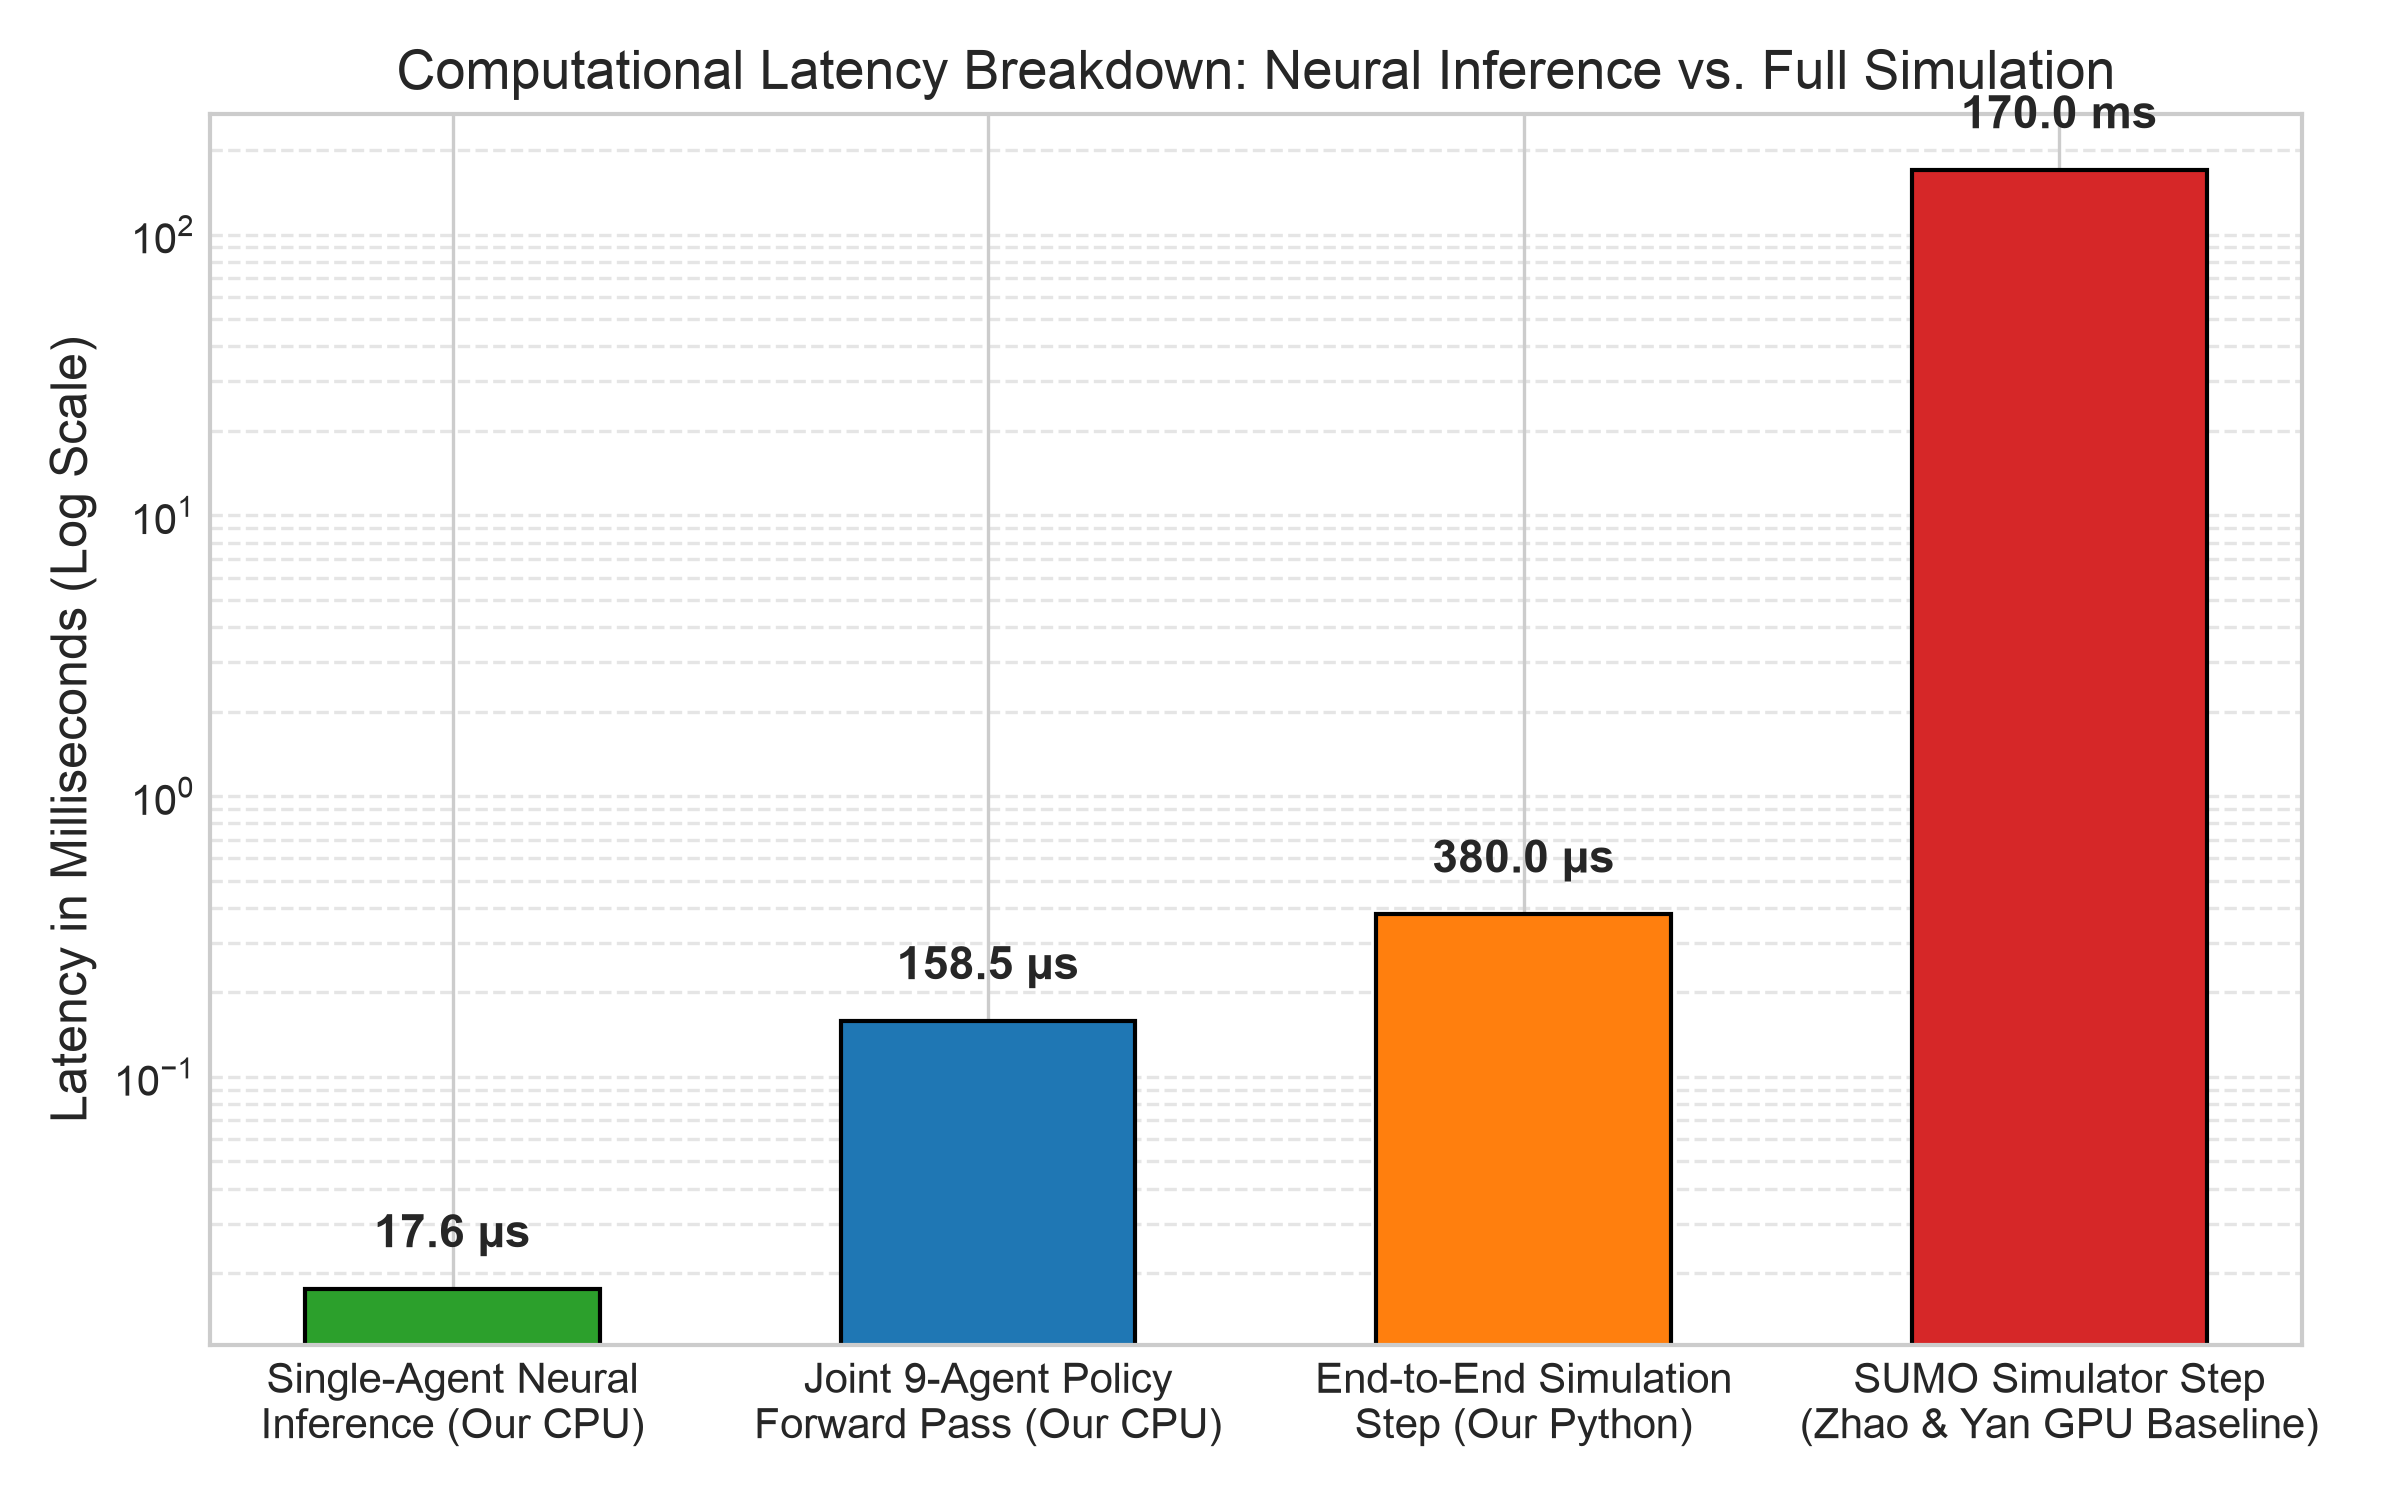
\includegraphics[width=0.88\linewidth]{figures/fig4_inference_latency_distribution.png}
\caption{Computational Latency Profiling: Isolated single-agent ($17.6~\mu$s) and joint 9-agent policy forward latency ($158.5~\mu$s) versus complete simulation cycle times (log scale).}
\label{fig:latency}
\end{figure}

\section{Discussion, Limitations \& Threats to Validity}

\subsection{Methodological Framing of Municipal Simulation}
The experimental simulator represents a \textbf{trace-calibrated discrete simulation} parameterized by City of Melbourne open sensor distributions ($\text{Gamma}(2.33, 18.58)$, 541 bays across 9 districts), rather than a live hardware-in-the-loop vehicle GPS replay. Engineering safeguards, including the 0.95 saturation cap and reward alignment, are disclosed adaptations necessary for numerical simulation stability.

\subsection{Threats to Validity}
We identify three primary threats to the empirical validity of this study:
\begin{itemize}
    \item \textbf{Internal Validity:} Multi-agent training was conducted under a 30-episode exploratory budget (3,600 environment transitions). While numerical stability (critic loss $\le 4.04$, Q-mean $11.98$) was formally achieved, full asymptotic policy convergence on high-dimensional graph topologies typically requires extended curriculum learning ($\ge 500$ episodes).
    \item \textbf{Construct Validity:} Cruising delay is modeled via the reciprocal non-linear queuing formula $\eta = e_p / (1 - \delta / \sigma)$. While theoretically established in transportation economics~\cite{shoup2006cruising}, real-world cruising duration also depends on traffic signal timings, turn delays, and driver visual scanning behavior not captured in macro-level queuing equations.
    \item \textbf{External Validity:} The municipal network comprises 9 aggregated district nodes in Melbourne. Generalizability to continuous micro-street networks or alternative metropolitan layouts requires empirical re-calibration of adjacency matrices and arrival priors.
\end{itemize}

\subsection{Limitations \& Future Work}
While our implementation provides numerical stability and sub-millisecond edge profiling, several open research directions remain:
\begin{enumerate}
    \item \textbf{Extended Curriculum Scaling:} Scaling training to 500+ episodes with prioritized experience replay to determine whether MARL-GCN can match or surpass deterministic FIFO under dynamic non-stationary surges.
    \item \textbf{Action Space Discretization:} Investigating discrete action parameterizations (e.g., Gumbel-Softmax or QMIX) to evaluate whether discrete selection mitigates continuous policy over-smoothing.
    \item \textbf{Simulation-to-Real Transfer:} Bridging the gap between the municipal 541-bay simulation and physical IoT testbeds (such as our 5-stall campus deployment) through domain adaptation.
\end{enumerate}

\section{Conclusion}
This paper presented an independent implementation, numerical stabilization, and empirical validation of a paper-aligned heterogeneous graph attention and hypernetwork MARL architecture for urban parking search navigation. By establishing Twin-Critic Clipped Double-Q evaluation, gradient norm clipping, and reward scaling, we resolved fundamental critic explosion in multi-agent continuous parking environments. Extensive benchmarking across 8 multi-tier scenarios ($N=10$ paired seeds, 240 simulations) confirmed robust allocation up to 900 vehicles, isolated the temporal GRU as the essential architectural component ($+545.5\%$ delay explosion when ablated, $p = 3.03 \times 10^{-6}$), demonstrated descriptive optimization overhead from attention on compact topologies under short horizons, and verified sub-millisecond edge latency ($158.5~\mu$s).

\bibliographystyle{IEEEtran}
\bibliography{references}

\end{document}
